\clearpage

\section{Comparing the Results}
\label{sec:comparing}

In this section, we will be comparing the results obtained by both the Theoretical Analysis and the Simulation.

In the following tables and plots, we can observe the results already presented in previous sections now side by side, with the first table being the result of the simulation and the second one being the result from the theoretical analysis. These are displayed in this
way as a means of easier representation.

\subsection{Table Comparison}


\begin{figure}[ht]
\centering
\begin{subfigure}{.5\textwidth}
  \centering
  \begin{tabular}{|l|r|}
  \hline    
  {\bf Variable} & {\bf Value (dB)} \\ \hline
  gaindbmax & 3.834218e+01\\ \hline

  \end{tabular}
  \begin{tabular}{|l|r|}
  \hline    
  {\bf Variable} & {\bf Value ($k\Omega$)} \\ \hline
  zin & 9.999982e+02,-3.99820e+02\\ \hline

 \end{tabular}
 \begin{tabular}{|l|r|}
  \hline    
  {\bf Variable} & {\bf Value ($k\Omega$)} \\ \hline
  zout & 8.011868e+02,-3.99270e+02\\ \hline

  \end{tabular}
\end{subfigure}%
\begin{subfigure}{.4\textwidth}
  \centering
  \begin{tabular}{|l|r|}
  \hline    
  {\bf Variable} & {\bf Value} \\ \hline
  \input{../mat/totalteo.tex}
  \end{tabular}
\end{subfigure}
\caption{Simulation Values (LEFT) and Theoretical Values (RIGHT)}
\label{fig:sbs1}
\end{figure}


In the tables above we can compare the gain (in dB), the input impedance (on the left - $k\Omega$, on the right - $\Omega$) and the output impedance (on the left - $k\Omega$, on the right - $\Omega$)).

\vspace{2cm}


\subsection{Plot Comparison}

\vspace{-3cm}

\begin{figure}[ht]
\centering
\begin{subfigure}{.5\textwidth}
  \centering
  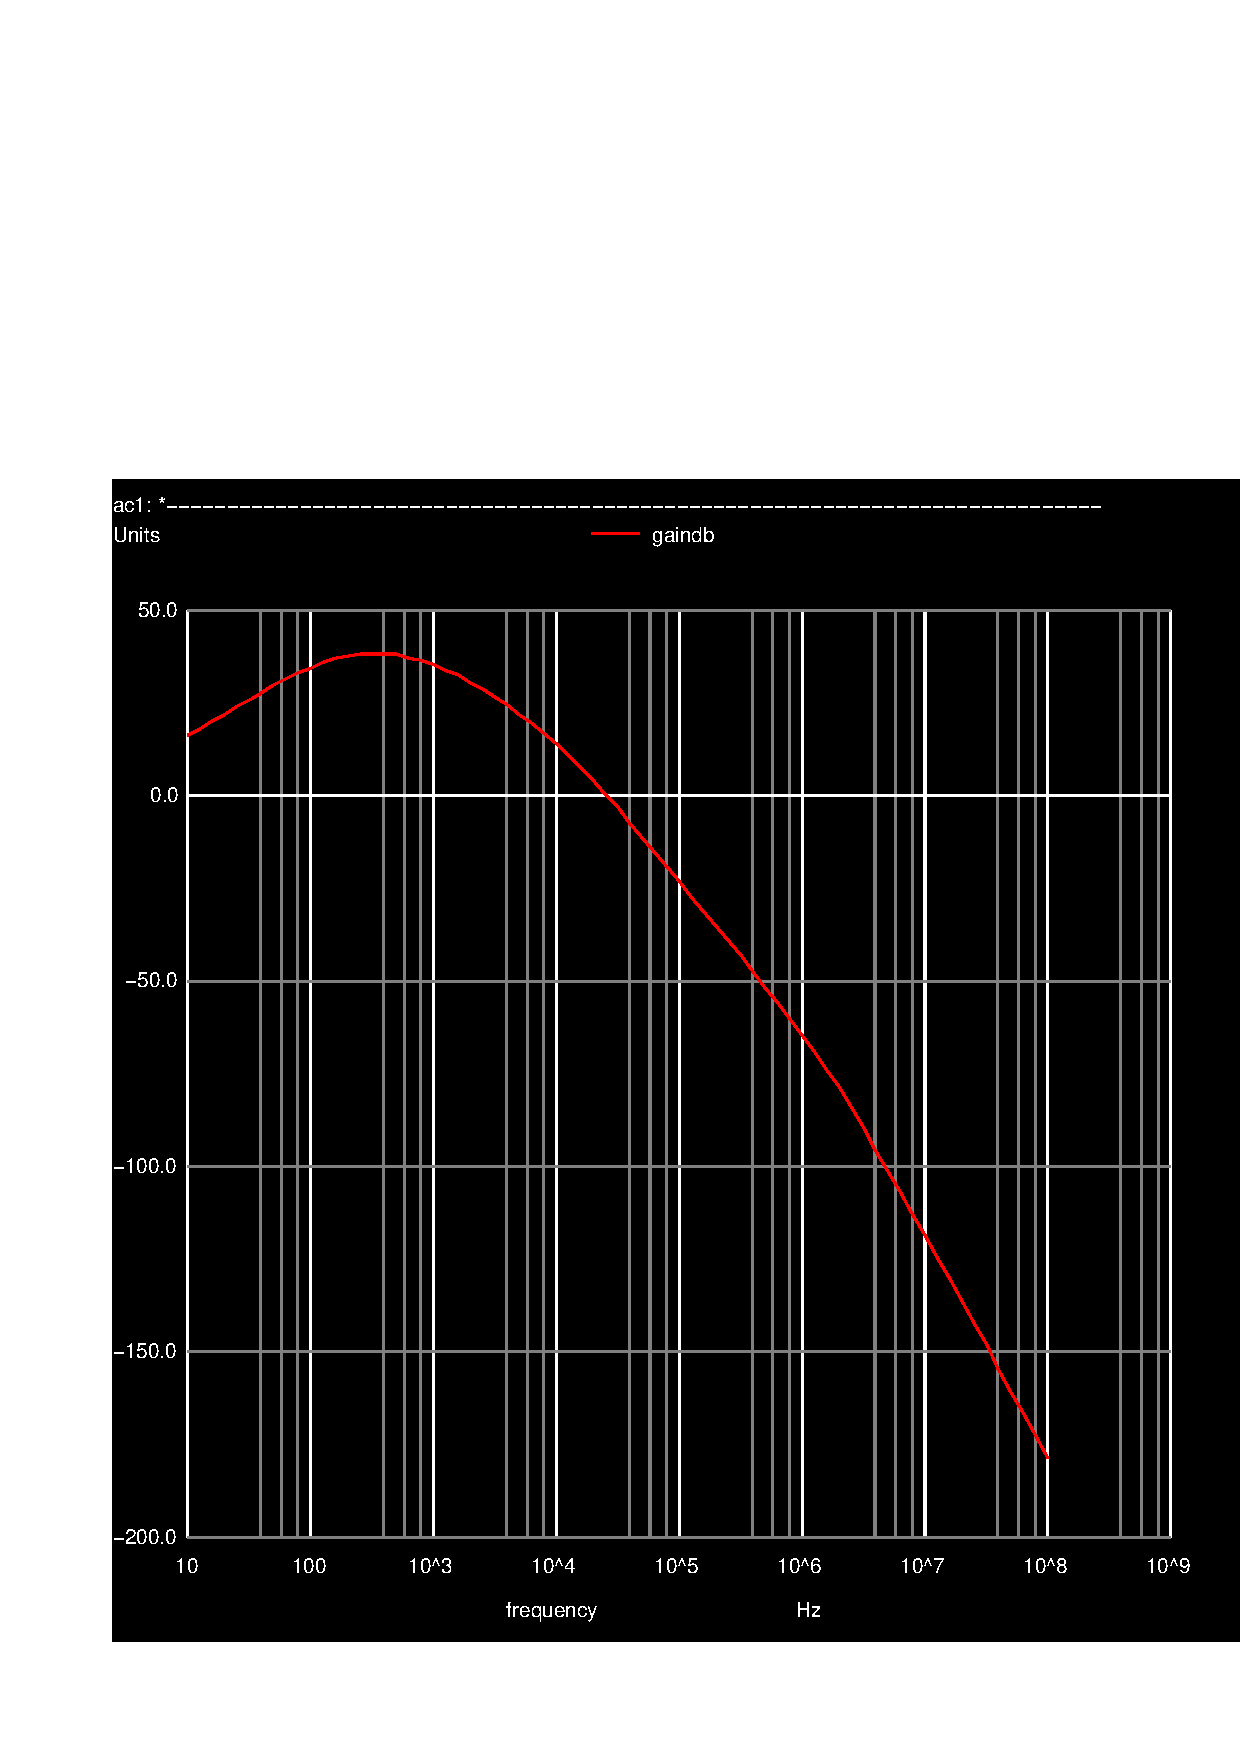
\includegraphics[width=0.9\linewidth]{../sim/gain.pdf}
\end{subfigure}%
\begin{subfigure}{.5\textwidth}
  \centering
  \vspace{3cm}
  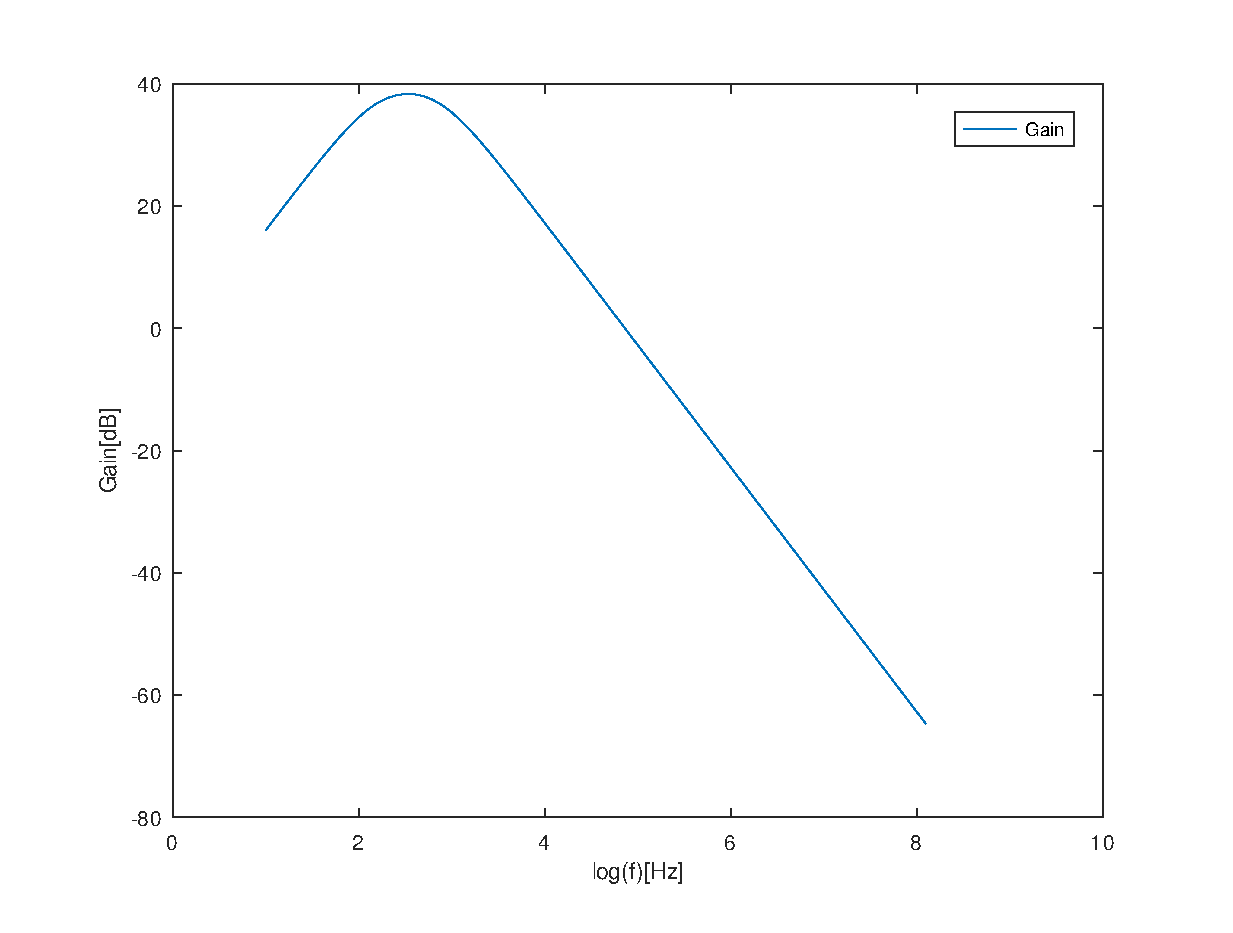
\includegraphics[width=1\linewidth]{gainteo.eps}
\end{subfigure}
\caption{Simulation Gain Values (LEFT) and Theoretial Gain Values (RIGHT)}
\label{fig:sbs3}
\end{figure}


Straightforwardly, we can verify that the theoretical plot, for low frequencies, closely resembles the plot obtained by simulation. However, for high frequencies the plots are clearly different. It's thought that, due to linear approximations, the theoretical model isn't ideal for highfrequency analysis, whereas the simulation, using non-linear components closer to reality, isn't prone to this kind of deviation.